\chapter{Kameramodel}
\label{sec:CameraModels}

Um eine Szenenrekonstruktionalgorithmus zu verstehen, werden in diesem Abschnitt grundlegende  Bedingungen eingeführt um die Bildaufnahme mathematisch zu beschreiben. Ein Abbildendes System besteht aus einem Objekt $M$, einer Kamera $C$ und einer Bildebene $I$ wie in Abbildung \ref{fig:PinholeCamera3D} dargestellt.\\

\begin{minipage}{\linewidth}
	\centering
	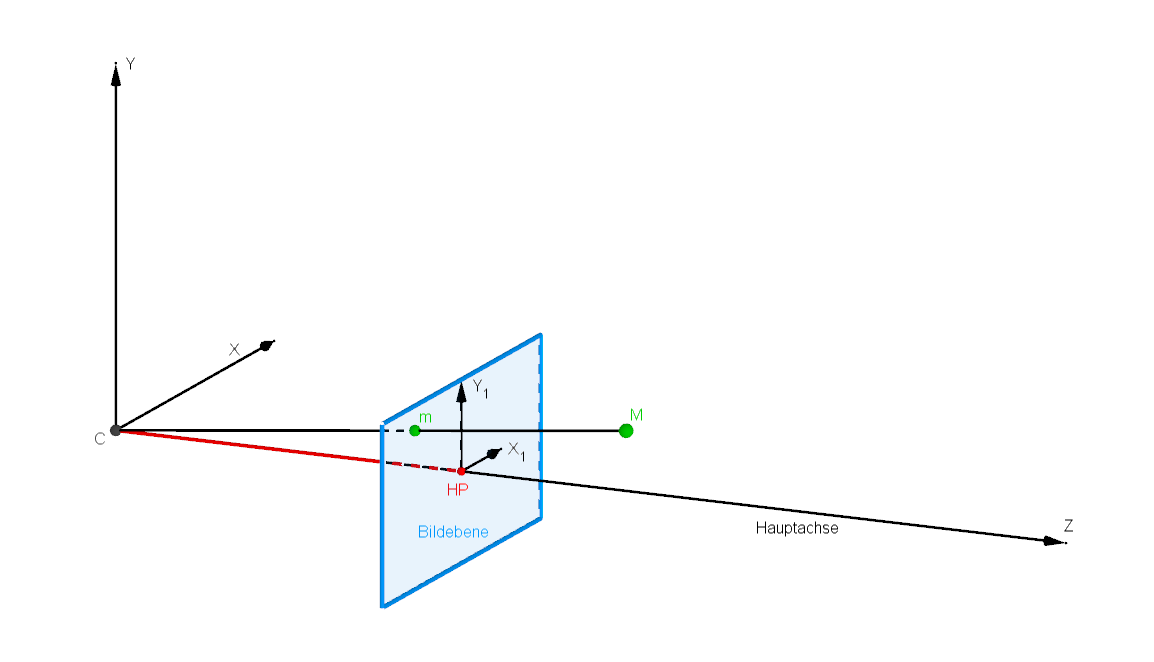
\includegraphics[width=.8\linewidth]{images/PinholeCameraModell3D.png}
	\captionof{figure}{Schematik eines Abbildendes System. Eine Punkt $M$ im  Weltkoordinatensystem wird durch eine Kamera $C$ aufgenommen. Diese Aufnahme wird durch eine Projektion, die als Verbindungslinie von $M$ zu $C$ dargestellt ist und $M$ auf $m$ abbildet, beschrieben. }
	\label{fig:PinholeCamera3D}
\end{minipage}\\\\

Ein Punkt $M$ in einem dreidimensionalen Weltkoordinatensystem wird mit Hilfe der Kamera, die in einem eigenen dreidimensionalen Kamerakoordinatensystem beschrieben wird, auf die Bildebene $I$ projiziert, welches durch ein zweidemensionales Bildkoordinatensystem beschrieben ist. Der projizierte Punkt $m$ kann mit einem Sensor aufgenommen und abgespeichert werden.  \\ 

Im folgenden wird zuerst ein Kameramodel eingeführt um die Projektion auf die Bildebene zu beschreiben. Daraufhin werden Koordinatentransformationen eingeführt um abschließend die Aufnahme eines Punktes mit einer willkürlichen Kameraorientierung zu berechnenS. 


\section{Lochkameramodell}

Mit Hilfe des Lochkameramodells wird die Abbildung eines Objektes auf die Bildebene beschrieben.
Das Modell beruht ausschließlich auf der geometrischen Optik und vernachlässigt physikalische Effekte wie Beugung oder die Auswirkung der Linse\cite{Heipke}. Das Lochkameramodell besteht aus einem Projektionszentrum $C$. $C$ beschreibt gleichzeitig die Lage des Kamerazentrums und bildet den Ursprung des Kamerakoordinatensystems.\cite{CamerModels.,HZ}.
Die Blickrichtung der Kamera wird als Hauptachse bezeichnet. Die Hauptachse ist auf eine Bildebene gerichtet. Der Schnittpunkt der Hauptachse mit der Bildebene wird Hauptpunkt $HP$ genannt. Der Hauptpunkt bildet den Ursprung des Bildebenenkooridnatensystems. Der Abstand vom Projektionszentrum zum Hauptpunkt wird als Brennweite $\zeta$ beschrieben\cite{HZ,CamerModels.}. Der Bildpunkt $m$ entsteht am Schnittpunk der Verbindungsgerade von $C$ und $M$ mit der der Bildebene $I$. 

\begin{minipage}{\linewidth}
	\centering
	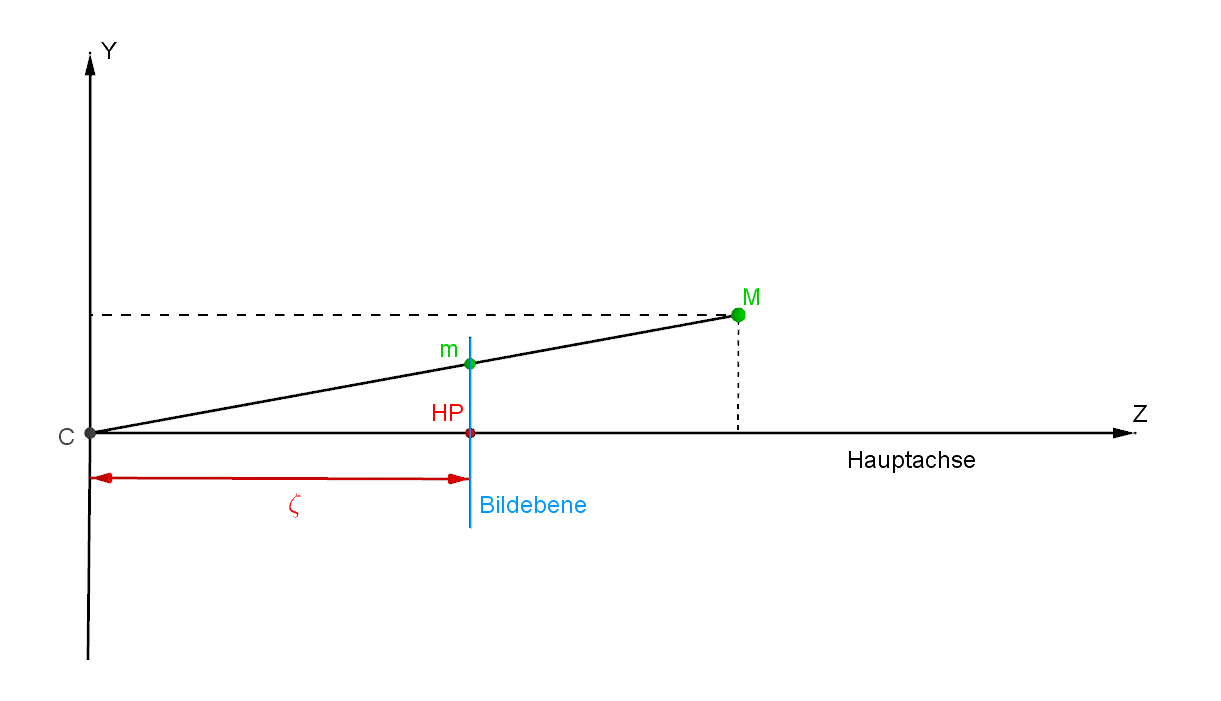
\includegraphics[width=.8\linewidth]{images/PinholeCameraModell2D.png}
	\captionof{figure}{Lochkameramodell \cite{Jianzhong}}
	\label{fig:PinholeCamera2D}
\end{minipage}\\ \\

Die Projektion eines dreidimensionalen Punktes auf eine zweidimensionale Bildebene, wird durch eine $3 \times 3$ Kameramatrix $K$ beschrieben. Die Kameramatrix beinhaltet alle Informationen über die intrinsischen Kameraparameter einer Kamera. $\zeta$ ist ein intrinsischer Kameraparameter. Mit $\zeta$ kann ein dreidimensionaler Punkt  $M=[X\,Y\,Z]$ in Kamerakoordinaten in einen Punkt $m$ in Bildebenenkoordinaten projiziert werden.

\begin{gather}
	K\cdot M =
	\begin{bmatrix}
		\zeta&0&0&0\\
		0&\zeta&0&0\\
		0&0&1&0
	\end{bmatrix}
	\cdot
	\begin{bmatrix}
		X\\Y\\Z
	\end{bmatrix}
=
	\begin{pmatrix}
	\zeta X\\ \zeta Y\\ Z
\end{pmatrix}
	\mapsto
	\begin{pmatrix}
		\zeta \frac{X}{Z}\\ \zeta \frac{Y}{Z}
	\end{pmatrix}
\end{gather}\\

Der Bildpunkt auf der Bildebene ist nur eine Vorstufe zum richtigen Bild. Die Bildpunkte auf der Bildebene werden im Sensor der Kamera gespeichert. Der Sensor wird durch die Bildebene dargestellt. Der Sensor wird in einem eigenen zweidimensionalen Sensorkoordinatensystem beschrieben, dessen Ursprung sich in einer Ecke der Bildebene befindet. Ein Sensor besteht aus einer Ansammlung von Pixel. Pixel sind die kleinsten Bausteine eines Bildes. Die geometrische Form eines Pixels kann sowohl quadratisch als auch rechteckig oder die Form eines Parallelogramm haben. Das Sensorkoordinatensystem passt seine Achsen der geometrischen Form eines Pixels an.\cite{HZ,CamerModels.}. Um einen Punkt $M$ in auf den Sensor zu pojizieren und den Bildpunkt dann in Sensorkoordinaten zu beschreiben, muss die Kameramatrix um weitere intrinsische Parameter erweitert werden. 

\begin{gather}
	K=\begin{bmatrix}
		\alpha_x&s&x_{0}\\
		0&\alpha_y&y_{0}\\
		0&0&1
	\end{bmatrix}
\end{gather}\\

Gleichung 2.2 beschreibt die erweiterte Kameramatrix $K$. Der Parameter $\zeta$, welcher zuvor für die Brennweite stand, wird in die Werte $\zeta_x$ und $\zeta_y$ unterteilt. Anstelle der Brennweite, beschreiben $\zeta_x$ und $\zeta_y$ den Abstand des Projektionszentrums zu den Kanten eines Pixels. Abbildung \ref{fig:focalLengthErklaerung} zeigt schematisch, dass $\zeta_x$ den horizontalen Abstand und $\zeta_y$ den vertikalen Abstand beschreibt\cite{HZ}.


\begin{minipage}{\linewidth}
	\centering
	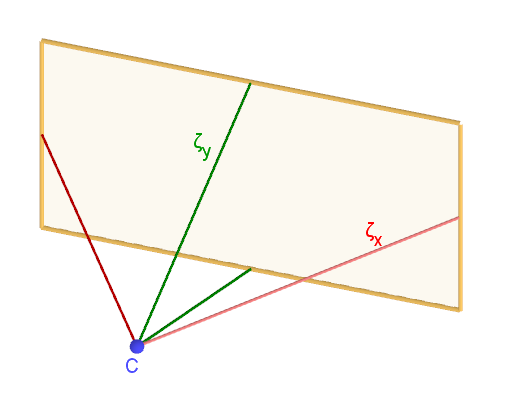
\includegraphics[width=.6\linewidth]{images/FocalLengthExplanation.png}
	\captionof{figure}{$\zeta_x$ und $\zeta_y$ beschreiben den Abstand des Kamerazentrums zu den jeweiligen Pixelkanten}
	\label{fig:focalLengthErklaerung}
\end{minipage}\\\\

Sind die Pixel quadratisch so sind $\zeta_x$ und $\zeta_y$ gleich. Sind die Pixel nicht quadratisch, wird $\zeta_x$ und $\zeta_y$ um die werte $k_x$ und $k_y$ skaliert\cite{HZ}.

\begin{gather*}
	\alpha_x = \zeta_x \cdot m_x\\
	\alpha_y = \zeta_y \cdot m_y
\end{gather*}

Die Matrixeinträge $p_x$ und $p_y$ beschreiben die Position des Hauptpunkts $HP$ bezüglich des Sensorkoordinatensysems. $p_x$ und $p_y$ müssen bei nicht-quadratischen Pixel auch um die Faktoren $k_x$ und $k_y$ skaliert werden\cite{HZ}.

\begin{gather}
	x_{0} = p_x \cdot m_x\\
	x_{0} = p_y \cdot m_y
\end{gather}

$s$ steht für den Schieflagefaktor. Trifft die Hauptachse der Kamera orthogonal auf den Bildsensor so ist $s = 0$. $s$ ändert seinen Wert zu $s \neq 0$, wenn die Hauptachse nicht mehr orthogonal auf den Bildsensor auftrifft\cite{HZ}. 

%\subsection{Lochkameramodell}
%\subsection{Kameramatrix}
\section{Koordinatentransformation}

Um ein Punkt von einem übergeordneten Weltkoordinatensystem in ein bestimmtes zum Weltkoordinatensystem verdrehtes Kamerakoordinatensystem zu überführen ist eine Transformation notwendig. Im folgenden wird der mathematische Weg einer Transformation eines Weltkoordinatensystem $(O,\delta)$ mit $\delta = (\hat{d_1},\hat{d_2},\hat{d_3},O)$ in ein Kamerakoordinatensystem $(C,\beta)$ = $\beta = (\hat{b_1},\hat{b_2},\hat{b_3},C)$ beschrieben.



\begin{minipage}{\linewidth}
	\centering
	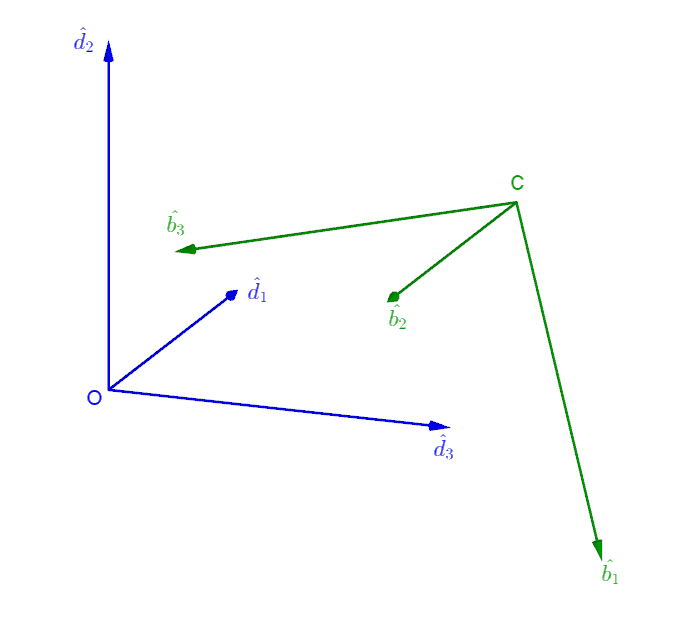
\includegraphics[width=0.7\linewidth]{images/WeltKordSys.png}
	\captionof{figure}{Weltkoordinatensystem $(O,\delta)$ mit $\delta = (\hat{d_1},\hat{d_2},\hat{d_3},O)$ und Kamerakoordinatensystem  $(C,\beta)$ mit $\beta = (\hat{b_1},\hat{b_2},\hat{b_3},C)$ }
	\label{fig:Koordinatensysteme1}
\end{minipage}\\ \\

Zunächst wird eine Koordinatisierung von Punkten im Weltkoordinatensystem vorgenommen. Ein Punkt $P_\delta$ bezüglich des Weltkoordinatensystems wird dann wie folgt beschrieben.


\begin{gather}
	P_\delta = O + p_{1\delta}\hat{d_1} + p_{2\delta}\hat{d_2} + p_{3\delta}\hat{d_3}\\
	\leadsto P_\delta = (p_{1\delta},p_{2\delta},p_{3\delta})^T = \begin{pmatrix} p_{1\delta} \\ p_{2\delta} \\ p_{3\delta} \end{pmatrix}
\end{gather}

Um das Koordinatentupel in einem projektiven Raum darstellen zu können, wird es projektiv erweitert. Die Entstehenden projektiv erweiterten Koordinaten werden als homogene Koordinaten bezeichnet. Ein Punkt $P_\delta$ bezüglich des Weltkoordinatensystems wird um eine vierte homogene Komponente erweitert. Diese kann einen Wert zwischen 0 und 1 annehmen. Nimmt die Komponente den Wert 0 an, so handelt es sich um einen Fernpunkt, sprich der Punkt liegt im unendlichen.
%wird dann zum Zweck der Einführung homogener Objekte projektiv Erweitert.

\begin{gather}
	P_\delta = \begin{bmatrix} p_{1\delta} \\ p_{2\delta} \\ p_{3\delta} \\1 \end{bmatrix} = \left\{ k \begin{bmatrix} p_{1\delta}\\p_{2\delta}\\p_{3\delta}\\1 \end{bmatrix} \in \mathbb{R} ^4 |  k \in \mathbb{R}\right\}\\
	\begin{bmatrix}\lambda p_{1\delta}\\ \lambda p_{2\delta} \\ \lambda p_{3\delta} \\ 1 \end{bmatrix} = \begin{bmatrix}p_{1\delta} \\ p_{2\delta} \\ p_{3\delta} \\ 1\end{bmatrix} \text{für} \; \lambda \ne 0
\end{gather}

\pagebreak
Ein Punkt $P_\beta$ bezüglich des Kamerakoordinatensystem wird im Vergleich wie folgt beschrieben.

\begin{gather}
	P_\beta = C + p_{1\beta}\hat{b_1} + p_{2\beta}\hat{b_2} +  p_{3\beta}\hat{b_3}\\
	P_\beta = \begin{pmatrix} p_{1\beta} \\  p_{2\beta} \\ p_{2\beta}\end{pmatrix}
\end{gather}\\

	Zwischen den beiden Koordinatensystemen	$(O,\delta)$  und $(C,\beta)$ werden die folgenden Beziehungsgleichungen aufgestellt. 

\begin{gather}
	C_\beta = O_\delta + C_{\beta,1}\hat{d_1} +C_{\beta,2}\hat{d_2} + C_{\beta,3}\hat{d_3}\\
	\hat{b_1} = b_{11}\hat{d_1} +  b_{12}\hat{d_2} +  b_{13}\hat{d_3}\\
	\hat{b_2} = b_{21}\hat{d_1} +  b_{22}\hat{d_2} +  b_{23}\hat{d_3}\\
	\hat{b_3} = b_{31}\hat{d_1} +  b_{32}\hat{d_2} +  b_{33}\hat{d_3}
\end{gather}

Diese Beziehungsgleichungen werden in Gleichung 2.5 eingesetzt.

\begin{gather}
	\begin{split}
		P_\delta = O + (C_{\beta,1} + p_{1\beta}b_{11} +  p_{2\beta}b_{21} + p_{3\beta}b_{31}) \cdot \hat{d_1}\\
		+(C_{\beta,2} + p_{1\beta}b_{21} +  p_{2\beta}b_{22} + p_{3\beta}b_{32} )\cdot \hat{d_2}\\
		+ (C_{\beta,3} + p_{1\beta}b_{31} +  p_{2\beta}b_{23} + p_{3\beta}b_{33} )\cdot \hat{d_3}
	\end{split}
\end{gather}

Aus Gleichung 2.15 wird ein Gleichungssystem in der Form von Gleichung 2.16 aufgestellt und gelöst.

\begin{gather}
	\begin{split}
		p_{1\delta} = C_{\beta,1} + (C_{\beta,1} + p_{1\beta}b_{11} +  p_{2\beta}b_{21} + p_{3\beta}b_{31} \\
		\leadsto \: p_{1\delta} - C_{\beta,1} =  (C_{\beta,1} + p_{1\beta}b_{11} +  p_{2\beta}b_{21} + p_{3\beta}b_{31})
	\end{split}
\end{gather}

Wenn $P_\beta$ gegeben ist, erhält man auf diese Weise direkt $P_\delta$. Wenn jedoch  $P_\delta$  gegeben ist, so muss das in Gleichung 2.17 aufgestellte lineare Gleichungssystem gelöst werden.

\begin{gather}
	\begin{bmatrix}b_{11} & b_{21} & b_{31}\\
		b_{12} & b_{22} & b_{32}\\
		b_{13} & b_{23} & b_{33}
	\end{bmatrix} 
	\begin{pmatrix}
		p_{1\beta}\\p_{2\beta}\\ p_{3\beta}
	\end{pmatrix} = 
	\begin{pmatrix}
		p_{1\delta} - C_{\beta,1}\\
		p_{2\delta} - C_{\beta,2}\\
		p_{3\delta} - C_{\beta,3}
	\end{pmatrix}
\end{gather}

Wenn $(C,\beta)$ ein kartesisches Koordinatensystem ist, so ist die entstehende  koeffizientenmatrix $D_\beta$ orthogonal und es gilt \ensuremath{D_\beta^{-1} = D_\beta^T}. 
\begin{gather}
	D_\beta^{T} = 
	\begin{bmatrix}b_{11} & b_{12} & b_{13}\\
		b_{21} & b_{22} & b_{23}\\
		b_{31} & b_{32} & b_{33}
	\end{bmatrix} \\
	\begin{split}
		\leadsto \: \begin{pmatrix}
			p_{1\beta}\\p_{2\beta}\\ p_{3\beta}
		\end{pmatrix}
		= D_\beta^T 
		\begin{pmatrix}
			p_{1\delta} - C_{\beta,1}\\
			p_{2\delta} - C_{\beta,2}\\
			p_{3\delta} - C_{\beta,3}
		\end{pmatrix}
	\end{split} 
\end{gather}

Handelt es sich um kein kartesisches Koordinatensystem, so muss lediglich die Inverse \ensuremath{D_\beta^{-1}} anstatt der Transponierten \ensuremath{D_\beta^T} gebildet und wie gehabt verfahren werden. Im folgenden wird noch einmal kompakt und in einer symbolischen Schreibweise die Transformation von Welt- in Kamerakoordinaten  festgehalten. Einmal wird wie bereits angefangen mit Spaltenvektoren gearbeitet, das selbe Verfahren wird dann noch einmal mit Zeilenvektoren dargestellt.  Beide Ansätze funktionieren nach dem selben Prinzip, der einzige Unterschied ist die Darstellung der Matrizen. Es ist jedoch gerade wenn man mit Programmen wie Beispielsweise \textit{Matlab} arbeitet wichtig zu wissen welche Darstellung benutzt wird und worin sie sich unterscheiden. Auf diese weise passieren keine Fehler beim Interpretieren der späteren Resultate. \textit{MatLab} arbeitet beispielsweise mit Spaltenvektoren, während im entstandenen Algorithmus dieser Arbeit mit Zeilenvektoren gearbeitet wurde. Zunächst wird also weiter mit Spaltenvektoren verfahren. Zur Erinnerung, es gilt, dass $\beta = (\hat{b_1},\hat{b_2},\hat{b_3},C)$ durch Rotation $D$ aus $\delta = (\hat{d_1},\hat{d_2},\hat{d_3},O)$ entstanden ist. Der Ursprung des Kamerakoordinatensystems ist bezüglich des Ursprungs des Weltkoordiantensystems verschoben. Zur Rotation des Koordinatesystems muss also auch noch eine Tranlation des Ursprungs durchgeführt werden. Der Translationsvektor ist gleich den Koordinaten des Ursprungs des Kamerakoordinatensystem $\vec{V} = C_\beta = (C_{\beta,1}, C_{\beta,2}, C_{\beta,3})^T$. Die Transformationsmatrix welche aus der Rotation $D$ und dem Translationsvektor $\vec{V}$ ensteht, wird im weiteren Verlauf mit $R$ bezeichnet. $R$ fasst die extrinsischen Kameraparameter in einer Matrix zusammen.

	\begin{gather}
	\begin{pmatrix}
		\hat{b_1}\\
		\hat{b_2}\\
		\hat{b_3}\\
		C_\beta
	\end{pmatrix} = 
	\begin{bmatrix}
		b_{11} & b_{21} & b_{31} & 0\\
		b_{12} & b_{22} & b_{32} & 0\\
		b_{13} & b_{23} & b_{33} & 0\\
		C_{\beta,1} & C_{\beta,2} & C_{\beta,3} & 1
	\end{bmatrix}
	\begin{pmatrix}
		\hat{d_1}\\
		\hat{d_2}\\
		\hat{d_3}\\
		O_\delta
	\end{pmatrix}\\
	D^T = D^{-1}= \begin{bmatrix}
		b_{11} & b_{12} & b_{13} \\
		b_{21} & b_{22} & b_{23} \\
		b_{31} & b_{32} & b_{33} 
	\end{bmatrix}\\
	D = \begin{bmatrix}
		b_{11} & b_{21} & b_{31} \\
		b_{12} & b_{22} & b_{32} \\
		b_{13} & b_{23} & b_{33} 
	\end{bmatrix}
\end{gather}

Für eine Rücktransformation von Kamera in Weltkoordinaten muss die Inverse von $D$ gebildet werden.
Außerdem muss der Translationsvektor $\vec{V}$ mit dieser Inversen multipliziert werden, um diesen in das Zielkoordinatensystem zu überführen.


\begin{gather}
	\leadsto \: \begin{pmatrix}
		\hat{d_1}\\
		\hat{d_2}\\
		\hat{d_3}\\
		O_\delta
	\end{pmatrix} = 
	\begin{bmatrix}
		b_{11} & b_{21} & b_{31} & 0\\
		b_{12} & b_{22} & b_{32} & 0\\
		b_{13} & b_{23} & b_{33} & 0\\
		&-(	C_{\beta,1}, C_{\beta,2}, C_{\beta,3})C^{-1}& & 1
	\end{bmatrix}
	\begin{pmatrix}
		\hat{b_1}\\
		\hat{b_2}\\
		\hat{b_3}\\
		C_\beta
	\end{pmatrix}
\end{gather}


Das selbe Verfahren mit Zeilenvektoren führt zu den Gleichungen 2.24 und 2.25.


\begin{gather}
	(\hat{b_1}, \hat{b_2}, \hat{b_3}, C_\beta) = (\hat{d_1},\hat{d_2}, \hat{d_3}, O) \cdot
	\begin{bmatrix} 
		b_{11} & b_{21} & b_{31} & C_{\beta,1}\\
		b_{12} & b_{22} & b_{23} & C_{\beta,2}\\
		b_{13} & b_{32} & b_{33} & C_{\beta,2}\\
		0           &       0       &   0         & 1   
	\end{bmatrix}
\end{gather}	

Daraus folgt, dass für den Fall der Rücktransformation gilt:

\begin{gather}
	\leadsto \: \begin{pmatrix}
		\hat{d_1},\hat{d_2},\hat{d_3},O
	\end{pmatrix} = 
	\begin{bmatrix}
		b_{11} & b_{12} & b_{13} & \\
		b_{21} & b_{22} & b_{23} &  -\begin{pmatrix}
			C_{\beta,1}\\
			C_{\beta,2}\\
			C_{\beta,3}
		\end{pmatrix}C^{-1}\\
		b_{31} & b_{32} & b_{33} & \\
		0&0&0 & 1
	\end{bmatrix}
	\begin{pmatrix}
		\hat{b_1},\hat{b_2},\hat{b_3},C_\beta
	\end{pmatrix}
\end{gather}	

\pagebreak


\section{Aufname mit einer willkürlichen Kameraorientierung}

Ein beliebiger Punkt im Weltkoordinatensystem kann mit der eingeführten Operation auf einen Sensor Projiziert werden. Es werden insgesamt vier verschiedenen Koordinatensysteme definiert.
Das Weltkoordinatensystem $(O,\delta)$ mit $\delta =(\hat{d_1}, \hat{d_2},\hat{d_3},O)$, das Kamerakoordinatensystem $(C,\beta)$ mit $\beta = (\hat{b_1},\hat{b_2},\hat{b_3},C)$, das Bildebenenkoordinatensystem $(I,\tau)$ mit $\tau = (\hat{t_1},\hat{t_2},I)$ und als letztes das Sensorkoordinatensystem mit $(S,\sigma)$ mit $\sigma = (\hat{u},\hat{v},S)$. Abbildung \ref{fig:KoordinatensystemeUeberblick} zeigt die Koordinatensysteme schematisch im Überblick. 


\begin{minipage}{\linewidth}
	\centering
	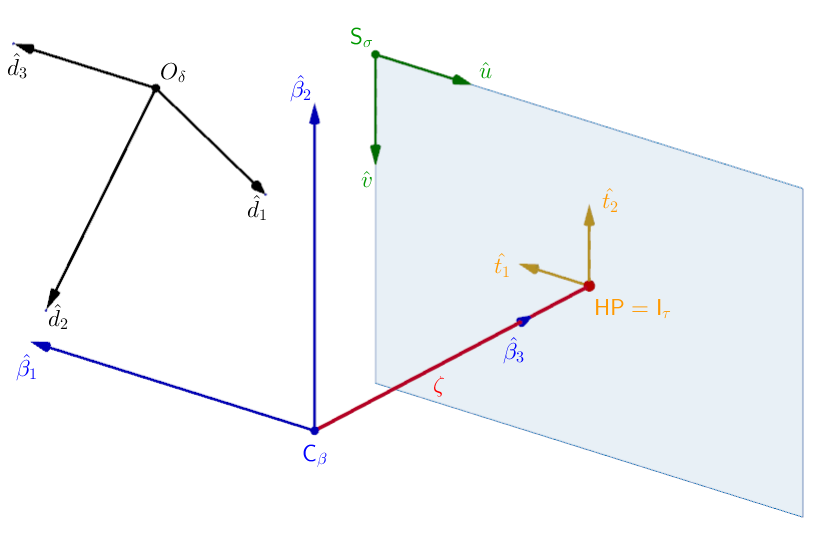
\includegraphics[width=0.8\linewidth]{images/UebersichtKoordinatensysteme_beschriftet.png}
	\captionof{figure}{Koordinatensysteme von einer Kamera aus im Überblick. Das Weltkoordinatensystem $(O,\delta)$ ist Deckungsgleich mit dem Kamerakoordinatensystem $(C,\beta)$}
	\label{fig:KoordinatensystemeUeberblick}
\end{minipage}\\ \\ 

Für die Projektion eines Punktes $M_\delta$ bezüglich des Weltkoordinatensystems in einen Punkt $m_\sigma$ bezüglich des Sensorkoordinatensystems, wir eine Projektionsmatrix $P$ definiert, welche sich aus den extrinsischen und intrinsischen Kameraparametern zusammensetzt. $P$ entsteht durch die Vereinigung der Transformationsmatrix $R$ und der Kamermatrix $K$\cite{HZ}.\\

Für die Transformation der Weltkoordinaten in Kamerakoordinaten gilt, dass $[\hat{d_1}\,\hat{d_2}\,\hat{d_3}\,1] \cdot R = [\hat{b_1}\,\hat{b_2}\, \hat{b_3}\, 1]$. $R$ bildet sich aus einer Rotationsmatrix $D$ und einem Translationsvektor $\vec{V}$, so das gilt $R = [D|V]$. Der Translationsvektor $\vec{V}$ setzt sich aus den Koordinaten des Projektionszentrums $C$ zusammen. Es gilt also $\vec{V} = C \leadsto \vec{v} = \begin{pmatrix}	C_{\delta,1}\\C_{\delta,2}\\C_{\delta,3}\end{pmatrix}$. 


%Das Weltkoordinatensystem $(O,\delta)$ und zwei Kamerakoordinatensysteme $(C,\beta)$, welche alle drei zu den dreidimensionalen Koordinatensystemen gehören. Des Weiteren gibt noch vier zweidimensionale Koordinatensysteme. Zum einen die Bildebenenkoordinatensystem $(I,\tau)$ und $(I',\tau')$ und die Sensorkoordinatensystem $(S,\sigma)$ und $(S',\sigma')$. Alle Koordinatensysteme sind innerhalb dieser Masterarbeit als kartesische, rechtsdrehende Koordinatensysteme festgelegt. Abbildung \ref{fig:KoordinatensystemeUeberblick} zeigt als Übersicht die Koordinatensysteme von einer Kamera ausgehend im Überblick. \\

%Das Weltkoordinatensystem $(O,\delta)$ ist mit $\delta = (\hat{d_1},\hat{d_2},\hat{d_3},O)$ definiert. Die Kamerakoordinatensysteme der Kameras werden mit $(C,\beta)$ mit $(\beta = \hat{b_1},\hat{b_2},\hat{b_3},C)$ und $(C',\beta')$ mit $(\hat{b_1}',\hat{b_2}',\hat{b_3}',C')$ bezeichnet. 
%
%Die Projektionszentren der Kameras entsprechen den Koordinatenursprüngen $C$ und $C'$, wie aus dem Lochkameramodell bekannt. Das zweidimensionale Bildebenenkoordinatensystem wird im weiteren Verlauf mit $(I,\tau)$ mit $\tau = (\hat{t_1},\hat{t_2},I)$ bezeichnet und zu guter Letzt fehlt noch das Sensorkoordinatensystem $(S,\sigma)$ mit $\sigma = (\hat{u},\hat{v},S)$.  Der Ursprung des Bildkoordinatensystem ist Deckungsgleich mit dem Hauptpunkt $HP$ auf der Bildebene. Der Ursprung des Sensorkoordinatensystems befindet sich in einer der Ecken der Bildebene. Das Bildebenenkoordinatensystem und das Sensorkoordinatensystem unterscheiden sich darin, dass das Sensorkoordinatensystem an die geometrie der Pixel auf dem Sensor angepasst ist und somit die Werte der Koordinatenachsen in Pixeleinheiten angegeben werden. Währendessen sind das Bildebenenkoordinatensystem, sowie auch die anderen hier vorgestellten Koordinatensysteme in dieser Arbeit immer in Millimeter definiert. Das Weltkoordinatensystem wird deckungsgleich mit dem Koordinatensystem von einer der beiden Kameras definiert, es gilt $(C,\beta)=(O,\delta)$.\\
%(Aufbau der Koordinatensyteme)



%Die komplette Projektionsmatrix $P=KR$\cite{HZ} besteht aus der Matrixmultiplikation der hergeleiteten Transformationsmatrix $R$ welche die externen Kamerparameter repräsentiert und der Kameramatrix $K$, welche die internen Kameraparameter repräsentiert\cite{HZ,ZZGXr}.
%
%
%Die Projektionsmatrizen $P$ und $P'$ bilden sich, aus den extrinsischen und intrinsischen Kameraparametern. Bei den extrinsischen Kameraparametern, handelt es sich um die jeweilige Orientierung einer Kamera bezüglich eines Weltkoordinatensystems, was in einer $3\times 4$-Transformationsmatrix $R$ beschrieben ist. $R$ kann sowohl eine Rotation als auch eine Translation beinhalten. Die intrinsischen Kameraparameter werden in der sogenannten Kameramatrix $K$ ausgedrückt. In der Literatur findet man diese wie folgt definiert\cite{HZ}.


%Nachdem die einzelnen Koordinatensysteme definiert sind, soll symbolisch die Projektion eines Objekts  aus dem 3D-Raum auf den 2D-Sensor aufgezeigt werden. Für die Transformation der Weltkoordinaten in Kamerakoordinaten gilt, dass $[\hat{d_1}\,\hat{d_2}\,\hat{d_3}\,1] \cdot R = [\hat{b_1}\,\hat{b_2}\, \hat{b_3}\, 1]$, wobei $R$ eine Tranformationsmatrix ist, wie sie im vorherigen Abschnitt eingeführt wurde. $R=[D|V]$, wobei $D$ eine $3 \times 3$-Rotationsmatrix darstellt und $V$ die Tranlationskomponente beschreibt. Der Translationsvektor \ensuremath{\vec{V}} besteht aus den Koordinaten des Projektionszentrums \textit{C}. Es gilt also $\vec{V} = C \leadsto \vec{v} = \begin{pmatrix}	C_{\delta,1}\\C_{\delta,2}\\C_{\delta,3}\end{pmatrix}$. 




\begin{gather} 		
	[\hat{b_1}, \hat{b_2}, \hat{b_3},1]=[\hat{d_1},\hat{d_2},\hat{d_3},1] \cdot
	\begin{bmatrix}
		&  &  &C_{\delta,1} \\
		&  [D]&  &C_{\delta,2} \\ 
		&  &  &C_{\delta,3} \\
		0&0&0 & 1
	\end{bmatrix}	
\end{gather}

Ein Punkt $M_\delta$ Mit $M_\delta=[X_\delta,Y_\delta,Z_\delta,1]$ wird mit der soeben aufgestellten Transformationmatrix $R=[D|V]$ zu einem Punkt $M_\beta$ bezüglich des Kamerakoordinatensystems transformiert.

\begin{gather}
	M_\beta = M_\delta \cdot R\\
	\begin{bmatrix}
		X_\beta& Y_\beta& Z_\beta&1\\
	\end{bmatrix} = 
	\begin{bmatrix}
		X_\delta& Y_\delta& Z_\delta&1\\
	\end{bmatrix} \cdot
	\begin{bmatrix}
		&  &  &C_{\delta,1} \\
		&  [D]&  &C_{\delta,2} \\ 
		&  &  &C_{\delta,3} \\
		0&0&0 & 1
	\end{bmatrix}	
\end{gather}


Nach der Transformation eines Punkte $M_\delta$ in 3D-Kamerakoordinaten zu $M_\beta$, erfolgt nun die Porjektion des 3D-Kamerapunktes $M_\beta$ in die 2D-Bildebene, so dass $M_\beta$ als Punkt $m_\tau$ bezüglich des Bildkoordinatensystems dargestellt wird. Für die Projektion wird eine $3 \times 3$-Kameramatrix $K_1$ aufgestellt, welche zunächst erstmal den Punkt $M_\beta$ zu einem auf der Bildebene $m_\beta$, jedoch noch bezüglich des Kamerakoordinatensystems darstellt.  

%Es wird angenommen, dass $\zeta_x = \zeta_y =\zeta$
%Im nächsten Schritt müssen die Transformierten Kamerakoordinaten noch mit einer entsprechenden Kameramatrix $K$, welche die Punkte aus dem Kamerakoordinatensystem $(C,\beta)$ auf das Koordinatensystem der Bildebene $(I,\tau)$ mit $\tau = (t_1,t_2)$ projiziert, verrechnet werden. Hierzu muss eine entsprechende Kameramatrix $K$ aufgestellt werden. $\zeta$ erhält als Wert den Abstand des Projektionszentrums $Z$ zur Bildebene $I$.

\begin{gather}
	K_1 = 
	\leftidx{_{{I_\beta}}}{\begin{bmatrix}
			\pi
	\end{bmatrix}}{_{{C_\beta}}}
	=
	\begin{bmatrix}
		\zeta&0&0&0\\
		0&\zeta&0&0\\
		0&0&\zeta&0\\
		0&0&1&0
	\end{bmatrix}\\
	\begin{bmatrix}
		\zeta&0&0&0\\
		0&\zeta&0&0\\
		0&0&\zeta&0\\
		0&0&1&0
	\end{bmatrix}
	\begin{bmatrix}
		X_\beta\\Y_\beta\\Z_\beta\\1
	\end{bmatrix} =
	\begin{pmatrix}
		\zeta X\\ \zeta Y\\ \zeta Z \\ Z
	\end{pmatrix}
	=
	\begin{bmatrix}
		\zeta \frac{X}{Z}\\ \zeta \frac{Y}{Z}\\ \zeta  \\ 1
	\end{bmatrix}
\end{gather}

%Für die Koordinaten der Bildebene $I_\beta$ ergeben sich dann aus den Kamerakoordinaten $[\zeta \frac{X}{Z},\zeta\frac{Y}{Z},\zeta,1]^T$.

Um Bildpunkt $m_\beta$ bezüglich des zweidimensionalen Bildebenenkoordinatensystems anzugeben, wird die Bildebene mit der Tiefen Komponente $\zeta$ normiert, so dass $m_\beta$ auf den zweidimensionalen Raum der Bildebene gemappt wird und der Bildpunkt $m_\tau$ mit $m_\tau = [\zeta \frac{X}{Z},\zeta\frac{Y}{Z},1]^T = [X_\tau, Y_\tau,1]$ entsteht.\\


Zuletzt folgt noch die Transformation der Bildebenenkoordinaten in die Sensorkoordinaten mit dem Sensorkoordinatensystem $(S,\sigma)$ mit $\sigma = (\hat{u},\hat{v},S)$. $\hat{u}$ und $\hat{v}$ definieren die geometrische Beschaffung der Pixel. Es wird angenommen, dass es sich um quadratische Pixel handelt. Für die Transformation wird eine Matrix $M$ aufgestellt, welche die Translation des Koordinatenursprungs und eine Skalierung der Koordinaten beinhaltet.


\begin{gather}	
k_x = \hat{u}\hat{t_1}\\
k_y = \hat{v}\hat{t_2}\\
S_\sigma = I_\tau + V_{\sigma,1} + V_{\sigma,2}\\
	m_\sigma = m_\tau \cdot M\\	
	m_\sigma = \begin{bmatrix}
		k_x&0&x_0\\
		0&k_y&y_0\\
		0&0&1
	\end{bmatrix} \cdot m_\tau 
\end{gather}


Die einzelnen Transformationsschritte, die ein Punkt bei einer Bildaufnahme durchläuft, können in einer einzigen Projektionsmatrix $P$ zusammengefasst werden. $P$ setzt sich zusammen aus der Transformationsmatrix $R$ und der erweiterten Kameramatrix $K$\cite{HZ,Ferid}.

\begin{gather}
	m_\sigma = P \cdot M_delta = MK_1R M_\delta = KR \cdot M_\delta
\end{gather}


